\newpage
{\samepage
\begin{center}
{\Large{\bf Simple Parsing}}
\end{center}
\begin{itemize}
\item Several fundamental algorithms have been developed
to recognise legal computer programs (or expressions) and to
decompose their structure into a form more suitable for processing.
\item This operation, know as parsing, has application
beyond Computer Science, since it is directly related to the study of
the structure of languages in general.
\end{itemize}
}


\newpage
{\samepage
\begin{center}
{\Large{\bf Infix Notation}}
\end{center}
{\small
\begin{itemize}
\item It is a long standing tradition in mathematics to write the operator
between the operands, as in \verb^x+y^, rather than \verb^x y +^.
\item The `normal' method with the operator between the operands is
known as {\it infix} notation.
\item As you scan a traditional infix expression, such as:
\begin{verbatim}
A+B/C+D
\end{verbatim}
from left- to right, it is impossible to tell when you initially encounter the \verb^+^ sign whether or not you should apply the indicated operation to
A.
\item You must probe deeper into the expression to determine whether an operation with a higher priority occurs.
\item This gets very complicated.
\item Brackets make this even worse.
\item The alternative is called {\it Postfix} or {\it Reverse Polish}
after the Polish logician J.\ Lukasiewicz (1958) who investigated the
properties of this notation.
\end{itemize}
}}

\newpage
{\samepage
\begin{center}
{\Large{\bf Reverse Polish Notation}}
\end{center}

Infix:
\begin{verbatim}
A+B*C
A*B+C
((A+B)*C+D)/(E+F+G)
\end{verbatim}

Reverse Polish
\begin{verbatim}
ABC*+
AB*C+
AB+C*D+EF+G+/
\end{verbatim}

Notice that no brackets are required in Reverse Polish. Therefore,
for simple applications, we could require the user to enter expressions
in postfix form.
}

\newpage
{\samepage
\begin{center}
{\Large{\bf Implementing Reverse Polish}}
\end{center}
\begin{itemize}
\item Reverse Polish may be evaluated by use of a stack.
\item Examine the next character;
\item If it is a number (or variable in the general case)
push it onto the stack.
\item If it is an operator (+-/*), pop off the top two
items, perform the operation and push the result.
\item If we have reached the end the answer is the one and only
item on the stack. Else repeat.
\begin{verbatim}
8 2 5 * + 1 3 2 * + 4 - /
\end{verbatim}
\end{itemize}

\begin{center}
\begin{tabular}{|c|c|c|c|c|c|c|c|c|}\hline
   & * & + &   & * & + & - &   & $/$ \\ \hline
   &   &   & 2 &   &   &   &   &     \\
 5 &   &   & 3 & 6 &   & 4 &   &     \\
 2 & 10&   & 1 & 1 & 7 & 7 & 3 &     \\
 8 & 8 & 18& 18& 18& 18& 18& 18& 6   \\ \hline
\end{tabular}
\end{center}
}

\newpage
{\samepage
\begin{center}
{\Large{\bf Implementing Reverse Polish}}
\end{center}
{\small
\begin{verbatim}
s = stack_init();
while(fgets(input, MAXINPUT, stdin)){
   /* If number push */
   if(sscanf(input, FORMATSTR, &d)==1){
      stack_push(s, d);
   }
   else{
      /* Must be an operator ? */
      assert(stack_pop(s, &g2));
      assert(stack_pop(s, &g1));
      switch(input[0]){
         case '+' :
            d = g1 + g2; break;
         case '-' :
            d = g1 - g2; break;
         case '*' :
            d = g1 * g2; break;
         case '/' :
            d = g1 / g2; break;
         default:
            fprintf(stderr, "Can't understand ? %d\n",
                    input[0]);
            exit(EXIT_FAILURE);
      }
      stack_push(s, d);
   }
}
assert(stack_pop(s, &d));
printf("Answer = ");
printf(FORMATSTR, d); printf("\n");
if(stack_peek(s, &d) == true){
   fprintf(stderr, "Stack still had items on it ?\n");
   exit(EXIT_FAILURE);
}
stack_free(s);
\end{verbatim}
}}

\newpage
{\samepage
\begin{center}
{\Large{\bf General Infix to Postfix}}
\end{center}
{\small
\begin{verbatim}
www.geeksforgeeks.org/stack-set-2-infix-to-postfix

Dijkstra's Shunting Yard Algorithm
==================================
1. Scan the infix expression from left to right. 
2. If the scanned character is an operand, output it. 
3. Else, 
  1 If the precedence of the scanned operator is
    greater than the precedence of the operator
    in the stack(or the stack is empty  or the
    stack contains a ‘(‘ ), push it. 
  2 Else, Pop all the operators from the stack
    which are greater than or equal to in
    precedence than that of the scanned
    operator.  After doing that Push
    the scanned operator to the stack.  (If you
    encounter parenthesis while popping then stop
    there and push the scanned operator in the
    stack.) 
4. If the scanned character is an ‘(‘, push it to the
   stack. 
5. If the scanned character is an ‘)’, pop the stack
   and and output it until a ‘(‘ is encountered, and
   discard both the parenthesis. 
6. Repeat steps 2-6 until infix expression is scanned. 
7. Print the output 
8. Pop and output from the stack until it is not
   empty.
\end{verbatim}
} }

\newpage
{\samepage
\begin{center}
{\Large{\bf Formal Grammars}}
\end{center}
\begin{itemize}

\item Parsing a program is the process of grammatically analysing how it is composed into parts.

\item Before we can write a program to determine whether a program
written in a given language is legal, we need a description of exactly
what constitutes a legal program.

\item Programming languages are often described by a particular type of
grammar called a {\it context free grammar}.

\end{itemize}
}

\newpage
{\samepage
\begin{center}
{\Large{\bf English}}
\end{center}
{\tiny Based on : \verb^web.stanford.edu/class/archive/cs/cs143/cs143.1128^}
{\small
\begin{verbatim}
<SENTENCE> ::= <SUBJECT> <VERB-PHRASE> <OBJECT>
<SUBJECT> ::= "This" | "Computers" | "I"
<VERB-PHRASE> ::= <ADVERB> <VERB> | <VERB>
<ADVERB> ::= "never"
<VERB> ::= "is" | "run" | "am" | "tell"
<OBJECT> ::= "the" <NOUN> | "a" <NOUN> | <NOUN>
<NOUN> ::= "university" | "world" | "cheese" | "lies"

This is a university.
Computers run the world.
I am the cheese.
I never tell lies.
\end{verbatim}
}}

\newpage
{\samepage
\begin{center}
{\Large{\bf Formal Grammars}}
\end{center}
\begin{itemize}

\item Say we wish to create a new computer language whose sole purpose
is to print out noughts and ones onto the screen~:

\begin{verbatim}
BEGIN
    ONE
    NOUGHT
    ONE
END
\end{verbatim}
\end{itemize}
}

\newpage
{\samepage
\begin{center}
{\Large{\bf 0's \& 1's Example}}
\end{center}
{\small
\begin{verbatim}
<PROG>      ::= "BEGIN" <CODE>
<CODE>      ::= "END" | <STATEMENT> <CODE>
<STATEMENT> ::= "ONE" | "NOUGHT"
\end{verbatim}
\begin{itemize}
\item The `\verb^|^' means OR.
\item \verb^"BEGIN"^, \verb^"ONE"^ and \verb^"NOUGHT"^ are string constants.
\item \verb^<CODE>^ is described recursively.
\item You could also think of this grammar in terms of a {\it railroad diagram}:
\begin{center}
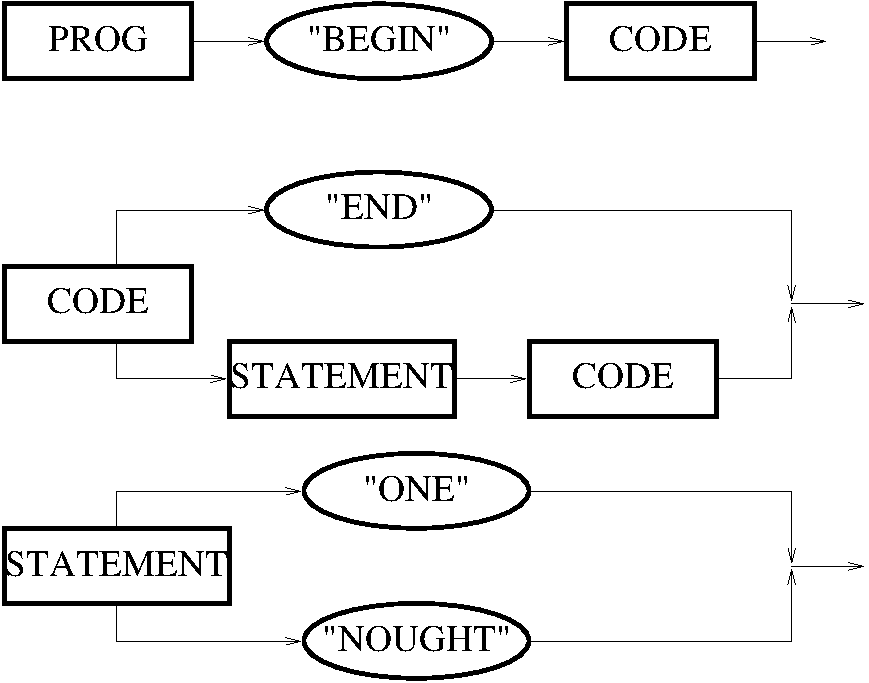
\includegraphics{../Images/railroad.pdf}
\end{center}
\end{itemize}
}}

\newpage
{\samepage
\begin{center}
{\Large{\bf 0's \& 1's Example}}
\end{center}
\begin{verbatim}
#include <stdio.h>
#include <string.h>
#include <stdlib.h>
#include <assert.h>

#define MAXNUMTOKENS 100
#define MAXTOKENSIZE 7
#define PROGNAME "01.no"
#define strsame(A,B) (strcmp(A, B)==0)
#define ERROR(PHRASE) {fprintf(stderr,
"Fatal Error %s occured in %s, line %d\n",
PHRASE, __FILE__, __LINE__); exit(2); }

struct prog{
   char wds[MAXNUMTOKENS][MAXTOKENSIZE];
   int cw; /* Current Word */
};
typedef struct prog Program;

void Prog(Program *p);
void Code(Program *p);
void Statement(Program *p);

\end{verbatim}
}

\newpage
{\samepage
\begin{center}
{\Large{\bf 0's \& 1's Example}}
\end{center}
\begin{verbatim}

int main(void)
{
   int i;
   FILE *fp;
   Program prog;

   prog.cw = 0;
   for(i=0; i<MAXNUMTOKENS; i++)
      prog.wds[i][0] = '\0';
   if(!(fp = fopen(PROGNAME, "r"))){
      fprintf(stderr, "Cannot open %s\n",
              PROGNAME);
      exit(2);
   }
   i=0;
   while(fscanf(fp, "%s", prog.wds[i++])==1
         && i<MAXNUMTOKENS);
   assert(i<MAXNUMTOKENS);
   Prog(&prog);
   printf("Parsed OK\n");
   return 0;
}
\end{verbatim}
}

\newpage
{\samepage
\begin{center}
{\Large{\bf 0's \& 1's Example}}
\end{center}
{\small
\begin{verbatim}

void Prog(Program *p)
{
   if(!strsame(p->wds[p->cw], "BEGIN"))
      ERROR("No BEGIN statement ?");
   p->cw = p->cw + 1;
   Code(p);
}

void Code(Program *p)
{
   if(strsame(p->wds[p->cw], "END"))
      return;
   Statement(p);
   p->cw = p->cw + 1;
   Code(p);
}

void Statement(Program *p)
{
   if(strsame(p->wds[p->cw], "ONE")){
      return;
   }
   if(strsame(p->wds[p->cw], "NOUGHT")){
      return;
   }
   ERROR("Expecting a ONE or NOUGHT ?");
}
\end{verbatim}
}}

\newpage
{\samepage
\begin{center}
{\Large{\bf 0's \& 1's Example}}
\end{center}
{\small
{\bf \begin{verbatim}
BEGIN
   ONE
   NOUGHT
   ONE
END
\end{verbatim}
}
\vspace*{-1.5ex}
Parsed OK

{\bf \begin{verbatim}
BEGIN ONE NOUGHT NOUGHT END
\end{verbatim} }
\vspace*{-1.5ex}
Parsed OK

{\bf \begin{verbatim}
BEGIN END
\end{verbatim} }
\vspace*{-1.5ex}
Parsed OK

{\bf \begin{verbatim}
BEGIN
  ONE
  TWO
END
\end{verbatim} }
\vspace*{-1.5ex}
Fatal Error Expecting a ONE or NOUGHT ?
occured in p01a.c, line 79

{\bf \begin{verbatim}
BEGIN
  ONE
  NOUGHT
\end{verbatim} }
\vspace*{-1.5ex}
Fatal Error Expecting a ONE or NOUGHT ?
occured in p01a.c, line 79

{\bf \begin{verbatim}
  ONE
  NOUGHT
END
\end{verbatim} }
\vspace*{-1.5ex}
Fatal Error No BEGIN statement ?
occured in p01a.c, line 55
}}

\newpage
{\samepage
\begin{center}
{\Large{\bf 0's \& 1's Example}}
\end{center}
{\small
\begin{itemize}
\item Notice that the END statement is actually used as the recursive base-case in the formal grammar in the function Code().
\item Notice that the parser doesn't actually do anything other than check that the input has the correct syntax.
\item An interpreter both checks the syntax and performs the required operations.
\item A slight modification to the code is required to produce an interpreter :
\end{itemize}
\begin{verbatim}
void Statement(Program *p)
{
   if(strsame(p->wds[p->cw], "ONE")){
      printf("1\n");
      return;
   }
   if(strsame(p->wds[p->cw], "NOUGHT")){
      printf("0\n");
      return;
   }
   ERROR("Expecting a ONE or NOUGHT ?");
}
\end{verbatim}
}}

\newpage
{\samepage
\begin{center}
{\Large{\bf Mathematical Expressions}}
\end{center}
To parse a string such as  "A+B*C", "A*(B+C)" or\\
"-(B*F)" we use :
\begin{verbatim}
<EXPR> ::= <EXPR><OP><EXPR> |
           "(" <EXPR> ")" |
           "-"<EXPR> | Letter
<OP>   ::= "+" | "-" | "*" | "/"

#include <stdio.h>
#include <ctype.h>
#include <stdlib.h>
#define MAXEXPR 400

struct prog{
        char str[MAXEXPR];
        int count;
};
typedef struct prog Prog;

void Op(Prog *p);
int isop(char c);
void Expr(Prog *p);
\end{verbatim}
}

\newpage
{\samepage
\begin{center}
{\Large{\bf Mathematical Expressions}}
\end{center}
{\small
\begin{verbatim}
int main(void)
{

   Prog p;
   p.count = 0;

   if(scanf("%[A-Z,+,-,*,/,(,)]s", p.str) != 1){
      printf("Couldn't read your expression ?\n");
      exit(2);
   }
   Expr(&p);

   printf("Parsed OK !\n");
   return 0;

}

int isop(char c)
{

   if(c=='+' || c=='-' || c=='*' || c=='/')
      return 1;
   else
      return 0;
}

void Op(Prog *p)
{
   if(!isop(p->str[p->count])){
      printf("I was expecting a letter ?\n");
      exit(2);
   }
}
\end{verbatim}
}}

\newpage
{\samepage
{\small
\begin{verbatim}
void Expr(Prog *p)
{
   if(p->str[p->count] == '('){
      p->count = p->count + 1;
      Expr(p);
      p->count = p->count + 1;
      if(p->str[p->count] != ')'){
         printf("I was expecting a ) ?\n");
         exit(2);
      }
   }

   else if(p->str[p->count] == '-'){
      p->count = p->count + 1;
      Expr(p);
   }

   /* Note Look-Ahead */
   else if(isop(p->str[p->count+1])){
      if(isupper(p->str[p->count])){
         p->count = p->count + 1;
         Op(p);
         p->count = p->count + 1;
         Expr(p);
      }
   }
   else{
      if(!isupper(p->str[p->count]) ||
         isupper(p->str[p->count+1])){
         printf("Expected a single letter ?\n");
         exit(2);
      }
   }

}
\end{verbatim}
}
}

\newpage
{\samepage
\begin{center}
{\Large{\bf Mathematical Expressions}}
\end{center}
{\bf \begin{verbatim}
A+(B*C)
\end{verbatim}}
Parsed OK !

{\bf \begin{verbatim}
-(B*C+D)
\end{verbatim}}
Parsed OK !

{\bf \begin{verbatim}
A
\end{verbatim}}
Parsed OK !

{\bf \begin{verbatim}
A+(C*
\end{verbatim}}
I was expecting a single letter ?

{\bf \begin{verbatim}
a+c
\end{verbatim}}
Couldn't read your expression ?

{\bf \begin{verbatim}
A*B+(C*D
\end{verbatim}}
I was expecting a ) ?
}

\newpage
{\samepage
\begin{center}
{\Large{\bf Mathematical Expressions}}
\end{center}
\begin{itemize}
\item The formal grammar doesn't explain everything that the
programmer needs to know.
\item It is not clear whether the \verb^a+c^ example is
invalid or not.
\item It is not clear how spaces should be dealt with.
\end{itemize}
}
